\documentclass{article}
\usepackage{graphicx} % Required for inserting images
\usepackage{placeins}
\title{Exploring Bayesian Statistics: A Review of 'Bayesian Statistics The Fun Way'}
\author{Shibo Liu}
\date{November 6th 2023}

\begin{document}

\maketitle

\section{Introduction}
The allure of Bayesian Statistics has captivated my intellectual curiosity for an extended duration. In the modern landscape, Bayesian Statistics plays an increasingly central role, extending beyond its traditional domain in Statistics and infiltrating cutting-edge technologies like artificial intelligence, particularly within the field of machine learning. As a graduate student in electrical and computer engineering, my statistical knowledge has predominantly revolved around frequentist methods. However, embarking on this project presents an invaluable opportunity to immerse myself in the intricacies of Bayesian Statistics. In this paper, I will expound upon various crucial concepts in Bayesian statistics, as elucidated in the book 'Bayesian Statistics The Fun Way,' and explore their potential applications.

\section{Revisit Bayes' Theorem}
The Bayes' Theorem can be derived from conditional probability, which refers to the probability of event A occurring when event B occurs, represented by $P(A|B)$.
\begin{figure}[!htbp]
    \centering
    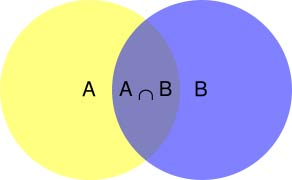
\includegraphics{Picture1.jpg}
    \caption{Venn Diagram of Two Events}
    \label{fig:enter-label}
\end{figure}
\FloatBarrier
According to the Venn diagram, it can be clearly seen that when event B occurs, the probability of event A occurring is $P(A \cap B)$ divided by P(B).
\[P(A|B)=\frac{P(A \cap B)}{P(B)}\]
Therefore,
\[P(A \cap B)=P(A|B)P(B)\]
Similarly,
\[P(A \cap B)=P(B|A)P(A)\]
Rearrange the equations, we could get the mathematical representation of Bayes' Theorem:
\[P(A|B)=\frac{P(A)P(B|A)}{P(B)}\]
The mathematical representation of Bayes' Theorem might not be immediately intuitive upon first glance. To better understand it, I would further explain it by highlighting the relationship between our observation and belief:\\\\
Let B denote belief and O denote observation.
\[P(B|O)=\frac{P(B)P(O|B)}{P(O)}\]
This formula can be split into four parts:
\begin{enumerate}
    \item $P(O|B)$: This component is commonly referred to as the likelihood function. It quantifies the probability of observing data (O) given our initial beliefs (B). Essentially, it measures how likely the observed event is based on our pre-existing understanding of the world.
    \item $P(B)$: This term is typically known as the prior function, representing our initial beliefs before taking any observations into account.
    \item $P(B|O)$: Commonly called the posterior function, it signifies the updated probability of our beliefs (B) after incorporating new evidence or observations (O). In essence, it reflects how our initial beliefs should be revised in light of the observed data.
    \item $P(O)$: This component signifies the total probability of observing a specific set of data, without regard to our initial beliefs or hypotheses. Within the framework of Bayes' theorem, it serves as a normalization factor, ensuring that the updated probability constitutes a valid probability distribution.
\end{enumerate}
One of the most captivating aspects of Bayes' Theorem lies in its unique capacity to merge our initial beliefs about the world with the empirical data we collect, resulting in an updated assessment of the reliability of our beliefs in light of the evidence at hand. This feature distinguishes Bayes' Theorem from traditional statistics, as traditional methods lack the ability to incorporate prior knowledge into their analyses.\\\\
In traditional statistics, the analysis primarily relies on observed data and typically excludes the explicit inclusion of prior beliefs or subjective information. However, when we leverage Bayes' Theorem in conjunction with our existing beliefs and observations, we empower ourselves to adapt our initial convictions and permit evidence to influence the strength of our beliefs.\\\\
Our initial beliefs are usually our starting level of confidence in an idea, represented as \(P(A)\) in Bayes' Theorem. Frequently, we engage in debates on subjects such as the climate change policies. But we may not always consider how new evidence should alter our perspectives or those of the individuals we are debating with.\\\\
Bayes' Theorem provides a framework for us to appraise the evidence related to these beliefs and to quantify precisely how this evidence should modify our convictions. This ability to update our beliefs in response to evidence is a cornerstone of Bayesian thinking, making it a powerful tool in fields like machine learning, medical diagnosis and so on.
\section{Apply Bayes' Theorem to Hypothesis Testing and Parameter Estimation}
\subsection{Hypothesis Testing}
The hypothesis testing is a fundamental component of statistical analysis. It begins by formulating two hypotheses: the null hypothesis and the alternative hypothesis. Data is collected, and a significance level is chosen to determine the threshold for statistical significance. A test statistic is then calculated based on the data and the null hypothesis, with the choice of test statistic depending on the specific test being conducted. The critical region, derived from the significance level and the test statistic's probability distribution, is defined to decide when to reject the null hypothesis. Comparing the test statistic to critical values, the null hypothesis is either rejected or not. The results are reported, including the test statistic's value and the decision made, often aided by the p-value, which quantifies the evidence against the null hypothesis. This traditional approach provides a structured methodology for evaluating hypotheses and drawing conclusions based on observed data but is limited in its dichotomous decision-making and the inability to directly incorporate prior knowledge.\\\\
With the introduction of Bayes Factor, we have a compelling alternative that offers several notable advantages. Bayes Factor leverages Bayes' Theorem, enabling us to assess hypotheses in a more nuanced and informative manner. Unlike the traditional approach, which often leads to a binary decision of either rejecting or failing to reject the null hypothesis, Bayes Factor quantifies the plausibility of competing hypotheses by directly comparing them. It provides a ratio that reveals how many times more likely one hypothesis is than another, effectively quantifying the strength of evidence in favor of one hypothesis over the other. This is particularly powerful as it allows for a continuous spectrum of evidence, making it a more flexible and informative tool for decision-making. Additionally, Bayes Factor readily incorporates prior knowledge, allowing for a seamless integration of existing beliefs with observed data. This capability for a richer and more probabilistic evaluation of hypotheses makes Bayes Factor a valuable addition to the statistical toolkit, offering a more versatile and robust approach to hypothesis testing.\\\\
Bayes Factor offers a flexible and probabilistic approach to hypothesis testing, providing a ratio that quantifies the strength of evidence for one hypothesis over another. While it has clear advantages, including the ability to incorporate prior knowledge and a more nuanced assessment of hypotheses, it comes with potential disadvantages. Sensitivity to prior choices and interpretation challenges can pose obstacles. Additionally, the appropriateness of Bayes Factor depends on the specific context and the comprehensiveness of the hypotheses being compared. Despite these limitations, it remains a valuable addition to the statistical toolkit, particularly when a richer and more informative analysis is desired.
\subsection{Parameter Estimation}
\end{document}
